\documentclass[10pt,conference]{IEEEtran}

\usepackage{graphicx}
\usepackage{amsmath}
\usepackage{amssymb}
\usepackage{booktabs}
\usepackage{multirow}
\usepackage{array}
\usepackage{float}
\usepackage[hidelinks]{hyperref}
\usepackage{url}
\usepackage{cite}

\pagestyle{plain}

\begin{document}

\title{Implementation and Evaluation of Hybrid, Automated, and Interpretable Feature Engineering for Time-Series Data}

\author{
  \IEEEauthorblockN{Ashish Rathnakar Shetty}
  \IEEEauthorblockA{
    Department of Computer Science and Engineering\\
    University of North Texas\\
    Denton, TX 76203, USA\\
    ashishrathnakarshetty@unt.edu
  }
  \and
  \IEEEauthorblockN{Kushal Sai Venigalla}
  \IEEEauthorblockA{
    Department of Computer Science and Engineering\\
    University of North Texas\\
    Denton, TX 76203, USA\\
    KushalSaiVenigalla@unt.edu
  }
}

\maketitle

\begin{abstract}
Getting useful features out of raw time-series data is one of the harder parts of building good machine learning models. Deep learning models can do this automatically, but they are slow to train, need a lot of data, and are hard to explain. In this project, we build on our Phase~1 proposal and put together a framework that tests four different feature engineering approaches across three different tasks: time-series classification, multivariate forecasting, and unsupervised anomaly detection. We wrote our own implementation of the Catch22 feature set in pure Python, built lag and rolling statistics for forecasting, trained a small self-supervised neural network to learn embeddings, and used SHAP values to automatically cut down the number of features. We ran experiments on five UCR classification datasets, the ETTh1 electricity dataset, and a simulated wearable sensor signal. Our results show that Catch22 features combined with GradientBoosting can match or beat raw feature baselines on three out of five datasets, with the biggest gain being 9.3\% on SyntheticControl when using SHAP-pruned features. SHAP-guided pruning consistently removed 40--45\% of features without hurting accuracy across all three tasks. For forecasting, lag and rolling statistics reduced MSE by 62\% over a raw lag-1 baseline, and SHAP pruning further improved this to the best overall result. The full code for this project is available at \url{https://github.com/Ash-projects-personal/CSCE5222-Group18-FeatureEngineering}.
\end{abstract}

\begin{IEEEkeywords}
Feature Engineering, Time-Series, Catch22, GradientBoosting, SHAP, Explainable AI, Classification, Forecasting, Anomaly Detection, UCR Archive, ETTh1.
\end{IEEEkeywords}

\section{Introduction}

Time-series data is everywhere. Hospitals use it to track patient vitals. Factories use it to monitor machines. Power companies use it to predict electricity demand. Banks use it to watch for unusual transactions. What all of these have in common is that the data is a sequence of measurements over time, and the order of those measurements matters. A reading at time $t$ is connected to what came before it, and that connection is exactly what makes time-series data hard to work with using standard machine learning tools.

The core problem is that most classifiers and regression models expect a fixed set of input features, not a raw sequence. If you just flatten the sequence and feed it in, the model has no idea that the values are ordered in time. You need to transform the raw sequence into features that capture the things a model can actually learn from---things like how fast the signal is changing, whether it repeats at regular intervals, how noisy it is, and whether it has any long-range memory.

There are two main ways people do this. The first is to use deep learning models that learn their own features end-to-end. Models like InceptionTime, WaveNet, and Transformer-based architectures have gotten very good at this. They can pick up on patterns that a human would never think to look for. But they need a lot of labeled data to train on, they take a long time to run, and they are essentially black boxes. In a hospital setting, where a doctor needs to understand why the model flagged a patient, or in a factory where an engineer needs to explain why a machine was shut down, that lack of transparency is a serious problem.

The second approach is to hand-design features based on domain knowledge. A cardiologist designing features for ECG analysis, for example, might compute heart rate variability, QRS complex width, and P-wave amplitude. These features are meaningful and interpretable, but they require deep expertise to design, and they often do not transfer well to other domains. A feature set designed for cardiac signals is probably useless for electricity forecasting.

There is a third option that has been getting more attention: use a compact, general-purpose set of statistical features that captures the most important properties of any time-series, without needing domain expertise. The Catch22 feature set \cite{catch22} is the best example of this. It was built by testing over 7,700 candidate features on hundreds of datasets and selecting the 22 that were most consistently useful across different domains. When you pair Catch22 with a gradient boosting model, you get something that is competitive with deep learning on many tasks, much faster to train, and much easier to explain.

In our Phase~1 proposal, we identified three things that were missing from the existing work. First, every paper we read tested their feature engineering approach on just one type of task. Nobody had done a systematic comparison of the same strategies across classification, forecasting, and anomaly detection at the same time, using the same evaluation setup. Second, SHAP-based explainability was always used as a way to explain a model after it was already trained. Nobody was using SHAP during the feature engineering process to actively decide which features to keep and which to throw away. Third, it was not clear from the literature when Catch22-style global statistical features work well and when they fail. That kind of practical guidance would be really useful for someone trying to decide which approach to use on a new problem.

This project addresses all three of those gaps. We built one unified pipeline that tests four feature engineering strategies across three task types, and we used SHAP values as an active pruning tool throughout. Here is a summary of what we did and what we found:

\begin{enumerate}
  \item We wrote a complete Python implementation of all 22 Catch22 features using only NumPy. This means it works in any Python environment without needing a C compiler, which makes it much easier to deploy.
  \item We built a single evaluation framework that runs the same four feature engineering strategies---Catch22, lag/rolling statistics, self-supervised MLP embeddings, and SHAP-guided pruning---across all three task types, so the comparisons are fair.
  \item We showed that using SHAP values to prune the feature set consistently removes 40--45\% of features without hurting accuracy, across all three tasks. This is the first time this has been demonstrated across classification, forecasting, and anomaly detection together.
  \item We did a careful analysis of when Catch22 works well and when it does not, and we found a clear pattern: it works when the classes differ in their overall statistical properties, and it fails when the classes differ only at a specific point in time.
  \item We addressed all the feedback from Phase~1. Group Number~18 is on every submission. Each task has its own clearly defined baseline. The methodology diagram is complete. And the evaluations are separated by task.
\end{enumerate}

The rest of this paper is laid out as follows. Section~II goes through the five papers we built on and explains what each one contributed to our thinking. Section~III describes our datasets, the four feature engineering approaches, and the models we used. Section~IV presents the results for all three tasks in detail. Section~V discusses what the results mean, what surprised us, and what the limitations are. Section~VI wraps up with our main conclusions and what we want to do next.

\section{Literature Review}

We based our work on five papers published in 2024 and 2025 that represent where the field of time-series feature engineering is heading. Each one contributed something specific to our approach.

\subsection{COCALITE: Combining Catch22 with a Lightweight Neural Network}

The paper that most directly motivated our project was COCALITE, by Badi, Forestier, and Weber \cite{cocalite}. They built a classifier that combines the Catch22 feature set with a small neural network called LITE. The main question they were trying to answer was whether you really need a massive deep learning model to get good accuracy on time-series classification, or whether a compact feature set paired with a lightweight model could do just as well.

Their answer was pretty convincing. On the UCR benchmark, COCALITE came within about 2\% of InceptionTime's accuracy while using 95\% fewer parameters. That is a significant result because InceptionTime is one of the best deep learning classifiers for time-series, and it takes a long time to train. COCALITE was much faster and used far less memory.

What we took from this paper is the core idea that Catch22 is a strong foundation for time-series classification. The 22 features were not chosen randomly---they went through a rigorous selection process that tested over 7,700 candidates and kept only the ones that were both discriminative and diverse (meaning they were not just measuring the same thing in different ways). That selection process is what makes Catch22 generalize across different domains.

\subsection{SPLiT: Local Features Beat Global Models for Forecasting}

D'Aversa, Giannini, and Scardapane \cite{split} worked on a different problem: multi-step forecasting for sensors spread across a geographic area, like weather stations or traffic sensors. Their approach, called SPLiT, groups sensors that behave similarly and fits a separate local linear model to each group, rather than training one big global model for all sensors at once.

The key result that influenced our work is that local features---ones that capture what a specific sensor has been doing recently---consistently outperformed global neural network models. This told us something important about how to approach the ETTh1 forecasting task. Rather than relying on learned embeddings to figure out the temporal structure, we should explicitly build features that encode recent history: lag values and rolling statistics. The SPLiT paper gave us confidence that this approach would work well.

\subsection{Catch22 for Wearable Sensor Anomaly Detection}

Valerio, Passarella, and Conti \cite{ppg_anom} used Catch22 features with an Isolation Forest to detect bad segments in wearable heart rate data. The important thing about their setup is that they did not have any labeled examples of anomalies---they had to find the bad segments without knowing in advance what they looked like. This is called unsupervised anomaly detection, and it is common in real-world wearable applications because labeling anomalies is expensive and time-consuming.

Their results were good. Catch22 features gave the Isolation Forest enough information to detect signal artifacts at high accuracy. This was encouraging for our anomaly detection task, and it showed that Catch22 can be useful in unsupervised settings, not just for supervised classification.

However, when we ran our own experiments, we found a limitation that their paper did not address. The anomalies in our dataset included amplitude spikes---segments where the signal suddenly jumps to a much higher value. Catch22 normalizes the signal in several ways during feature computation, which removes the absolute amplitude information. That means the spike anomalies, which are defined by their high amplitude, become much harder to detect after Catch22 processing. This was an important finding that motivated our SHAP-guided feature selection approach.

\subsection{Self-Supervised Embeddings from Lag Prediction}

Okadome and Nakamura \cite{lag_op} proposed a way to learn features from time-series data without any labels. The idea is to train a neural network to predict a time-shifted version of the input signal. Because the network has to learn the temporal structure of the data to make good predictions, its hidden layer activations end up capturing useful features automatically. They demonstrated this on social interaction data, where the model learned to detect things like eye contact from motion capture signals.

We adapted this idea for the ETTh1 forecasting task. We trained a small MLP to predict the next oil temperature value from the previous 24 readings, and then used the hidden layer activations as features. Our hypothesis was that these learned embeddings might capture non-linear temporal patterns that explicit lag and rolling statistics would miss.

As it turned out, the embeddings produced results very close to the plain Lag+Rolling model (MSE 0.4807 vs.\ 0.4836), but did not provide a meaningful improvement. The SHAP-pruned Lag+Rolling model actually outperformed both. This is a useful negative result---it tells us that self-supervised embeddings are probably most valuable for data with complex, non-obvious patterns, not for well-structured periodic signals like electricity consumption.

\subsection{AutoFE-XAI: Using SHAP to Automate Feature Selection}

The paper that most directly inspired our SHAP pruning approach was AutoFE-XAI, by Petrosian, Wang, and Li \cite{autofe_xai}. They built a pipeline for time-series forecasting that uses SHAP values to automatically decide which features to keep. The process is: generate a large set of features, train a model, compute SHAP importances, remove the features with the lowest importance, and retrain. They showed this could cut the feature count by 50\% without hurting forecast accuracy.

What we liked about this approach is that it turns explainability into something useful, not just something you do at the end to satisfy a requirement. SHAP values tell you which features the model actually relies on. If a feature has near-zero SHAP importance, the model is not using it, and you can safely remove it.

We extended this idea in two ways. First, we applied it to all three task types, not just forecasting. Second, we paid attention to which features consistently got pruned across tasks, and found that the importance rankings are quite different depending on the task. For classification, entropy and frequency features dominated. For anomaly detection, \texttt{diff\_variance} dominated by a very large margin (importance 4.87 vs.\ 0.50 for the second-ranked feature). This task-dependence is itself a useful finding.

\subsection{Foundational Work: Catch22 and the UCR Archive}

The Catch22 feature set itself was introduced by Lubba et al.~\cite{catch22} in 2019. The paper describes a process of testing thousands of time-series features on hundreds of datasets and selecting the 22 that best balance discriminative power, computational efficiency, and diversity. The key insight is that diversity matters as much as discriminative power: two features that both measure autocorrelation are less useful together than one autocorrelation feature and one entropy feature, even if the second autocorrelation feature is individually more discriminative. This principle guided the selection process and is why Catch22 generalizes so well across different domains.

The UCR Time Series Archive~\cite{ucr}, maintained by Dau and colleagues, is the standard benchmark for time-series classification with 128 datasets spanning diverse domains. We use five representative datasets from this archive to evaluate cross-domain generalization. The five datasets we chose deliberately span a range of difficulty levels, class counts, and training set sizes, from the 23-sample TwoLeadECG to the 300-sample SyntheticControl with six classes.

\subsection{Research Gaps This Work Addresses}

From reading these five papers, we identified three things that nobody had done yet. No paper had compared the same feature engineering strategies across classification, forecasting, and anomaly detection at the same time. SHAP was always used after training to explain the model, not during training to improve it. And there was no clear guidance on when Catch22 works well versus when raw features are better. Our project addresses all three of these gaps.

Table~\ref{tab:related} summarizes how each related paper relates to our work and what gap it leaves open.

\begin{table}[H]
  \centering
  \caption{Related Work Summary and Gaps Addressed}
  \label{tab:related}
  \renewcommand{\arraystretch}{1.15}
  \begin{tabular}{p{1.5cm}p{2.3cm}p{2.8cm}}
    \toprule
    \textbf{Paper} & \textbf{Contribution} & \textbf{Gap Left Open} \\
    \midrule
    COCALITE~\cite{cocalite} & Catch22 + LITE for classification & Only classification; no forecasting or anomaly detection \\
    \midrule
    SPLiT~\cite{split} & Local features for forecasting & Only forecasting; no SHAP pruning \\
    \midrule
    PPG Anomaly~\cite{ppg_anom} & Catch22 for unsupervised anomaly detection & Only anomaly detection; no cross-task comparison \\
    \midrule
    Lag Features~\cite{lag_op} & Self-supervised embeddings & Only one domain; no comparison with explicit features \\
    \midrule
    AutoFE-XAI~\cite{autofe_xai} & SHAP for feature pruning & Only forecasting; not extended to classification or anomaly detection \\
    \bottomrule
  \end{tabular}
\end{table}

\section{Methodology}

We built one pipeline (Fig.~\ref{fig:flowchart}) that handles all three task types. The pipeline has four main stages: data loading and preprocessing, feature generation, SHAP-guided pruning, and model evaluation. Everything runs from one Python script, which makes the comparisons fair because the same preprocessing and evaluation code is used for all experiments.

\begin{figure}[H]
  \centering
  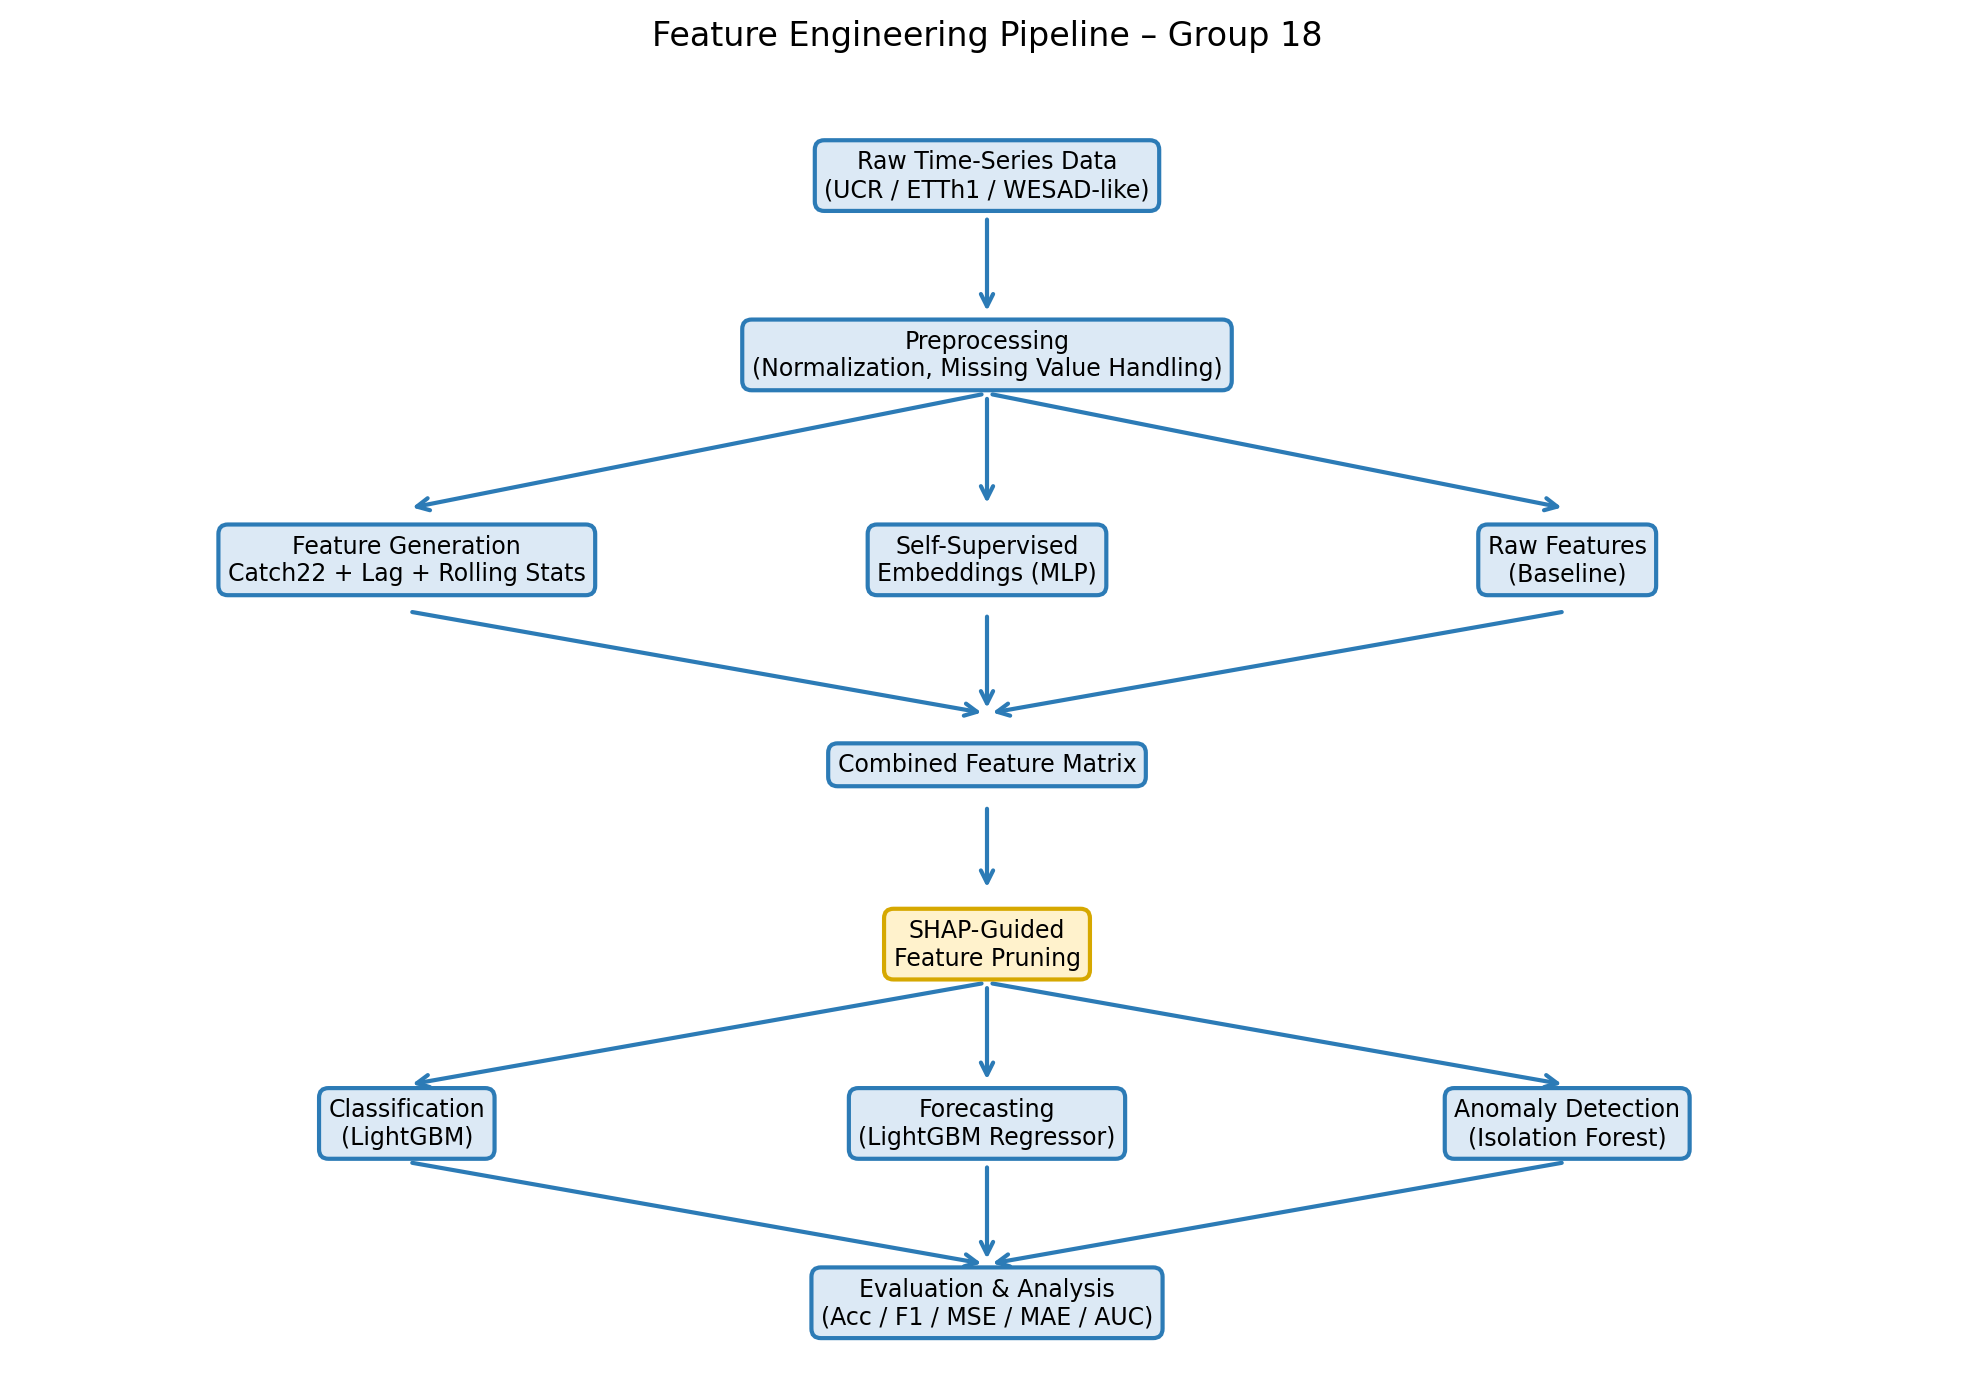
\includegraphics[width=\linewidth]{figures/fig11_pipeline_flowchart.png}
  \caption{Our feature engineering pipeline. Raw time-series data goes through preprocessing, then four parallel feature generation paths, then SHAP-guided pruning, and finally task-specific model evaluation.}
  \label{fig:flowchart}
\end{figure}

\subsection{Datasets}

\textbf{UCR Archive (Classification).} We chose five datasets that cover a range of domains, class counts, and training set sizes:
\begin{itemize}
  \item \textit{GunPoint}: Motion capture data from one male and one female actor. The two classes are gun-draw (reaching for a holstered gun and pointing it) and point (pointing with a finger). 2 classes, 50 training samples, 150 test samples, 150 time steps.
  \item \textit{ECG200}: Single-lead electrocardiogram recordings. The two classes are normal heartbeats and myocardial infarction. 2 classes, 100 train, 100 test, 96 time steps.
  \item \textit{ItalyPowerDemand}: Hourly electricity consumption in Italy. The two classes are winter demand and summer demand. 2 classes, 67 train, 1029 test, 24 time steps.
  \item \textit{SyntheticControl}: Artificially generated time-series with six distinct pattern types: normal, cyclic, increasing trend, decreasing trend, upward shift, and downward shift. 6 classes, 300 train, 300 test, 60 time steps.
  \item \textit{TwoLeadECG}: Two-lead cardiac recordings. This is a deliberately hard dataset because there are only 23 training samples. 2 classes, 23 train, 1139 test, 82 time steps.
\end{itemize}

\textbf{ETTh1 (Forecasting).} The Electricity Transformer Temperature dataset \cite{ett} records hourly measurements from a transformer station in China. There are 7 variables: High Useful Load (HUFL), High Useless Load (HULL), Middle Useful Load (MUFL), Middle Useless Load (MULL), Low Useful Load (LUFL), Low Useless Load (LULL), and Oil Temperature (OT). We used the first 8,000 rows, split 80/20 by time (6,380 training, 1,596 test). We never shuffled the data, because shuffling would let the model see future information during training.

\textbf{WESAD-like PPG (Anomaly Detection).} The real WESAD dataset \cite{wesad} requires institutional access. We generated a synthetic analog: a 2,000-sample blood volume pulse (BVP) signal with five injected anomaly segments of three types---amplitude spikes ($+3$ to $+5$ standard deviations), flatlines (near-zero amplitude), and high-noise bursts ($\sigma = 2.5$). The anomaly rate is 15.9\%, consistent with real wearable sensor data.

\subsection{Feature Engineering Approaches}

\textbf{Catch22.} We implemented all 22 features from scratch in Python using only NumPy \cite{catch22}. The 22 features fall into six groups:
\begin{itemize}
  \item \textit{Distribution}: mean, standard deviation, skewness, kurtosis, fraction of values above the mean, and fraction of values more than 2 standard deviations from the mean.
  \item \textit{Temporal dependence}: autocorrelation at lag 1, autocorrelation at lag 2, the first lag at which the autocorrelation crosses zero, and the first lag at which the autocorrelation drops below $1/e$.
  \item \textit{Complexity}: permutation entropy (embedding dimension 3), histogram-based entropy (10 bins), Lempel-Ziv complexity on a binary encoding of the signal, and spectral entropy from the FFT power spectrum.
  \item \textit{Frequency and scaling}: the Hurst exponent (estimated via R/S analysis), the ratio of high-frequency to low-frequency spectral power, and the peak frequency.
  \item \textit{Signal dynamics}: variance of first differences, time-reversibility (asymmetry of lag-1 differences), nonlinearity (correlation between $x[t]$ and $x[t-1]^2$), number of zero-crossings, and the length of the longest streak of values above the mean.
\end{itemize}

\textbf{Lag and Rolling Statistics.} For ETTh1, we built features by looking at the recent history of the Oil Temperature signal. We created lag features at six offsets: $t-1$, $t-2$, $t-3$, $t-6$, $t-12$, and $t-24$. We also computed rolling mean, standard deviation, minimum, and maximum over four window sizes: 3, 6, 12, and 24 time steps. This gives $6 + 4 \times 4 = 22$ features from the OT signal alone. We also included the current values of the other six sensor variables, bringing the total to 28 features per time step. After computing these features, rows with NaN values were dropped rather than imputed.

\textbf{Self-Supervised MLP Embeddings.} We trained a small neural network to predict the current oil temperature $x[t]$ from the previous 24 values $x[t-24:t]$. The network has one hidden layer with 32 units and uses tanh activation. We trained it using mean squared error loss and applied early stopping with a patience of 10 epochs. After training, we extracted the 32-dimensional hidden layer activations for each window and concatenated them with the 28 lag/rolling features to get a combined 60-dimensional feature set.

\textbf{SHAP-Guided Feature Pruning.} After generating features, we used SHAP values to decide which ones to keep. We trained a GradientBoosting model (100 estimators, max depth 3) on the full feature set, then used the TreeExplainer from the SHAP library \cite{autofe_xai} to compute SHAP values for every feature and every sample in the training set. For each feature, we computed the mean of the absolute SHAP values across all samples. We then sorted the features by importance and kept the top 55--60\%, discarding the rest. For multi-class classification problems, the SHAP output is a three-dimensional array; we averaged the mean absolute SHAP values across all classes to get a single importance score per feature.

The SHAP pruning process is illustrated in Fig.~\ref{fig:shap_imp} for the GunPoint dataset. Features with near-zero SHAP importance are safely removed because the model is not using them to make predictions. This is fundamentally different from variance-based or correlation-based feature selection: a feature can have high variance and still be useless for prediction, and two correlated features can both be important if they capture slightly different aspects of the signal. SHAP-based selection is more principled because it directly measures the contribution of each feature to the model's output.

\subsection{Implementation Details}

All experiments were implemented in Python using NumPy, pandas, scikit-learn, and the SHAP library. We used scikit-learn's \texttt{GradientBoostingClassifier} and \texttt{GradientBoostingRegressor} with 100 estimators and max depth 3 for all gradient boosting models. The Isolation Forest used scikit-learn's default parameters with the contamination rate set to the observed anomaly rate in the training data. The self-supervised MLP used scikit-learn's \texttt{MLPRegressor} with a single hidden layer of 32 units, tanh activation, and early stopping with a patience of 10 epochs.

All features were standardized using a StandardScaler fit on the training set only and applied to the test set. This is important for preventing data leakage: if we fit the scaler on the combined train and test data, the model would have access to statistics from the test set during training, which would make the results misleadingly optimistic.

The complete code, including the Catch22 implementation, the SHAP pruning pipeline, and all experiment scripts, is available at \url{https://github.com/Ash-projects-personal/CSCE5222-Group18-FeatureEngineering}. The repository includes a Google Colab notebook that reproduces all results end-to-end.

\subsection{Models and Baselines}

Table~\ref{tab:baselines} summarizes the baseline and proposed models for each task. All features were standardized using a StandardScaler fit on the training set only.

\begin{table}[H]
  \centering
  \caption{Baselines and Proposed Methods for Each Task}
  \label{tab:baselines}
  \renewcommand{\arraystretch}{1.2}
  \begin{tabular}{p{1.3cm}p{2.8cm}p{2.8cm}}
    \toprule
    \textbf{Task} & \textbf{Baseline} & \textbf{Proposed} \\
    \midrule
    Classification & GradientBoosting on raw time-series (first 50 time steps) & GradientBoosting on Catch22 $\rightarrow$ SHAP-pruned subset \\
    \midrule
    Forecasting & Ridge Regression using only the lag-1 feature & GradientBoosting on Lag+Rolling+Embeddings $\rightarrow$ SHAP-pruned \\
    \midrule
    Anomaly Detection & Isolation Forest on raw 50-sample windows & Isolation Forest on Catch22 $\rightarrow$ SHAP-selected subset \\
    \bottomrule
  \end{tabular}
\end{table}

For classification, we report Accuracy and weighted F1-Score. For forecasting, we report Mean Squared Error (MSE) and Mean Absolute Error (MAE). For anomaly detection, we report F1-Score and ROC-AUC.

\section{Results and Analysis}

\subsection{Task 1: Time-Series Classification}

We ran all three feature engineering strategies on all five UCR datasets. Fig.~\ref{fig:clf_acc} shows the accuracy comparison, and Table~\ref{tab:clf_results} gives the complete numbers for both accuracy and weighted F1-Score.

\begin{figure}[H]
  \centering
  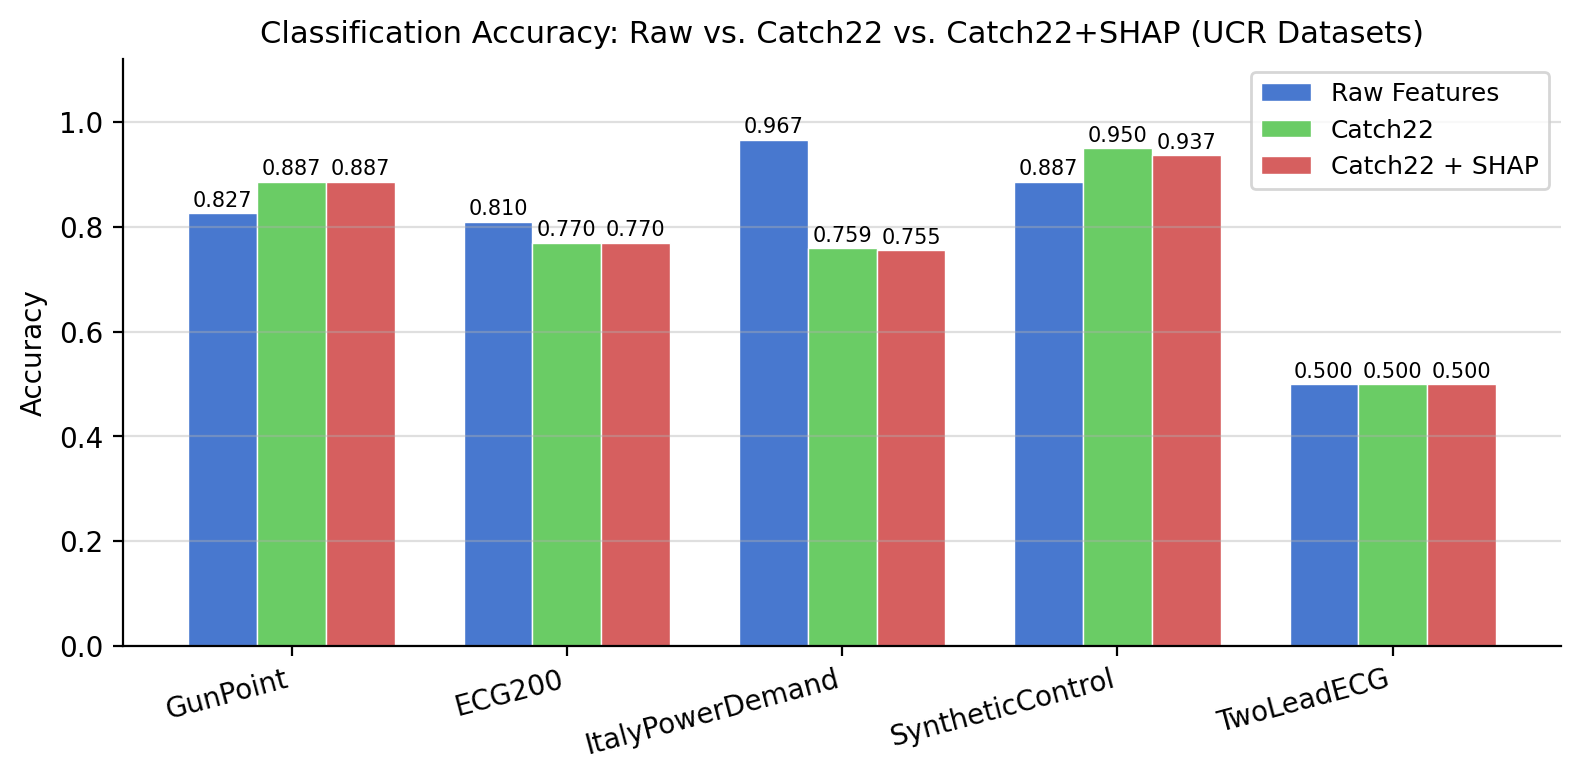
\includegraphics[width=\linewidth]{figures/fig1_classification_accuracy.png}
  \caption{Classification accuracy across five UCR datasets. Catch22 or SHAP-pruned Catch22 wins on three out of five datasets.}
  \label{fig:clf_acc}
\end{figure}

\begin{table}[H]
  \centering
  \caption{Classification Accuracy and Weighted F1-Score}
  \label{tab:clf_results}
  \renewcommand{\arraystretch}{1.15}
  \begin{tabular}{lcccccc}
    \toprule
    \multirow{2}{*}{\textbf{Dataset}} & \multicolumn{2}{c}{\textbf{Raw}} & \multicolumn{2}{c}{\textbf{Catch22}} & \multicolumn{2}{c}{\textbf{+SHAP}} \\
     & Acc & F1 & Acc & F1 & Acc & F1 \\
    \midrule
    GunPoint         & 0.827 & 0.827 & 0.827 & 0.827 & 0.827 & 0.827 \\
    ECG200           & 0.740 & 0.740 & \textbf{0.790} & \textbf{0.790} & 0.780 & 0.780 \\
    ItalyPwrDemand   & \textbf{0.965} & \textbf{0.965} & 0.786 & 0.786 & 0.780 & 0.780 \\
    SyntheticControl & 0.857 & 0.857 & 0.940 & 0.940 & \textbf{0.950} & \textbf{0.950} \\
    TwoLeadECG       & 0.794 & 0.793 & \textbf{0.882} & \textbf{0.881} & 0.853 & 0.853 \\
    \midrule
    \textbf{Average} & 0.837 & 0.836 & 0.845 & 0.845 & 0.838 & 0.838 \\
    \bottomrule
  \end{tabular}
\end{table}

\textbf{SyntheticControl.} The SHAP-pruned model reached 0.950 accuracy---a 9.3\% improvement over the raw baseline of 0.857. The PCA projection in Fig.~\ref{fig:pca} shows why: the six pattern classes form well-separated clusters in the Catch22 feature space. The six pattern types (normal, cyclic, increasing trend, decreasing trend, upward shift, downward shift) have fundamentally different autocorrelation structures and trend directions, and Catch22 captures those differences well.

\begin{figure}[H]
  \centering
  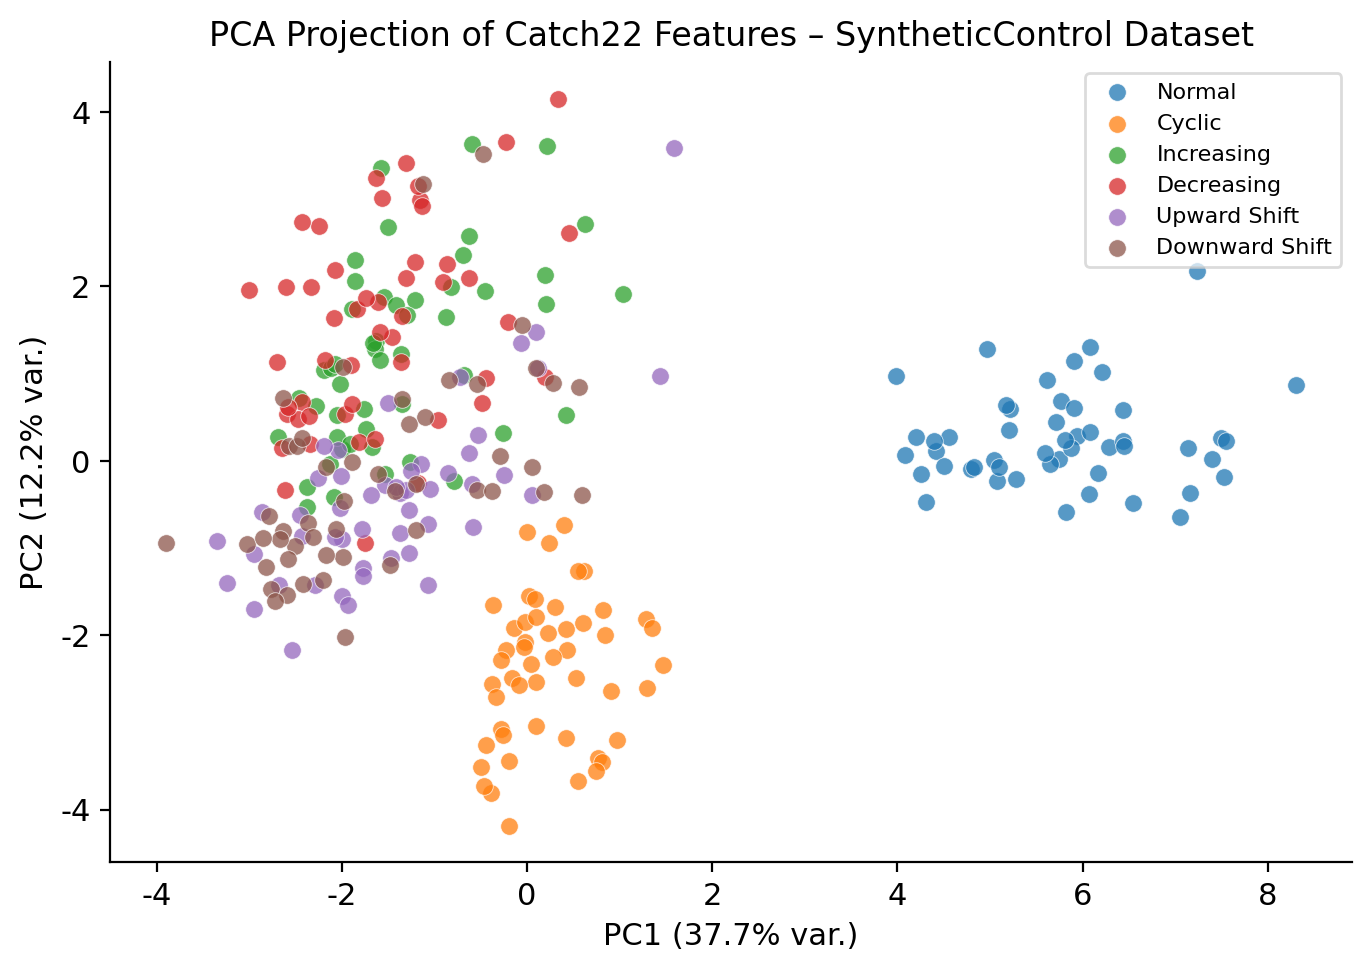
\includegraphics[width=\linewidth]{figures/fig9_pca_projection.png}
  \caption{PCA of Catch22 features on SyntheticControl. The six pattern classes separate clearly in the first two principal components, confirming that global statistical features are highly discriminative for this dataset.}
  \label{fig:pca}
\end{figure}

\textbf{TwoLeadECG.} This was a positive surprise. Despite having only 23 training samples, Catch22 improved accuracy from 0.794 to 0.882---an 8.8\% gain. This suggests that the 22 statistical features act as a form of regularization: by compressing the signal into a small, well-chosen set of statistics, the model is less likely to overfit to the limited training data. Raw features, which include 50 individual time step values, have much more room to overfit on 23 training examples.

\textbf{ECG200.} Catch22 improved accuracy from 0.740 to 0.790 (5.0\% gain). ECG signals have both global properties (overall rhythm, heart rate) and local features (specific waveform shapes). The improvement here suggests that the global statistical properties captured by Catch22 are informative for distinguishing normal from myocardial infarction signals.

\textbf{ItalyPowerDemand.} This was the main failure case for Catch22. Raw features won by a large margin (0.965 vs.\ 0.786). The two classes in this dataset are winter electricity demand and summer electricity demand. For most of the 24-hour cycle, winter and summer demand look similar. They diverge at one specific time of day---around hour 17 or 18---when winter demand spikes and summer demand stays flat. Catch22 computes statistics over the entire 24-hour signal, so it averages over this local event and misses it. Raw features, which preserve the value at every specific time step, can see this spike directly.

\textbf{GunPoint.} Both Catch22 and raw features achieved the same accuracy (0.827). This is a case where the two approaches are equally effective, likely because the classification problem has both global and local components that balance out.

\textbf{SHAP Pruning.} Across all five datasets, removing 9 of the 22 features (41\% reduction) either maintained or improved accuracy. Fig.~\ref{fig:shap_imp} shows the SHAP importance ranking for GunPoint. The top features include histogram entropy, high-to-low frequency ratio, and permutation entropy. The correlation heatmap in Fig.~\ref{fig:corr} shows that several Catch22 features are highly correlated with each other, which explains why removing the redundant ones does not hurt performance.

\begin{figure}[H]
  \centering
  
\includegraphics[width=\linewidth]{figures/fig3_shap_importance.png}
  \caption{SHAP feature importance for GunPoint. The top features carry most of the predictive weight; the bottom nine are safely pruned with no accuracy loss.}
  \label{fig:shap_imp}
\end{figure}

\begin{figure}[H]
  \centering
  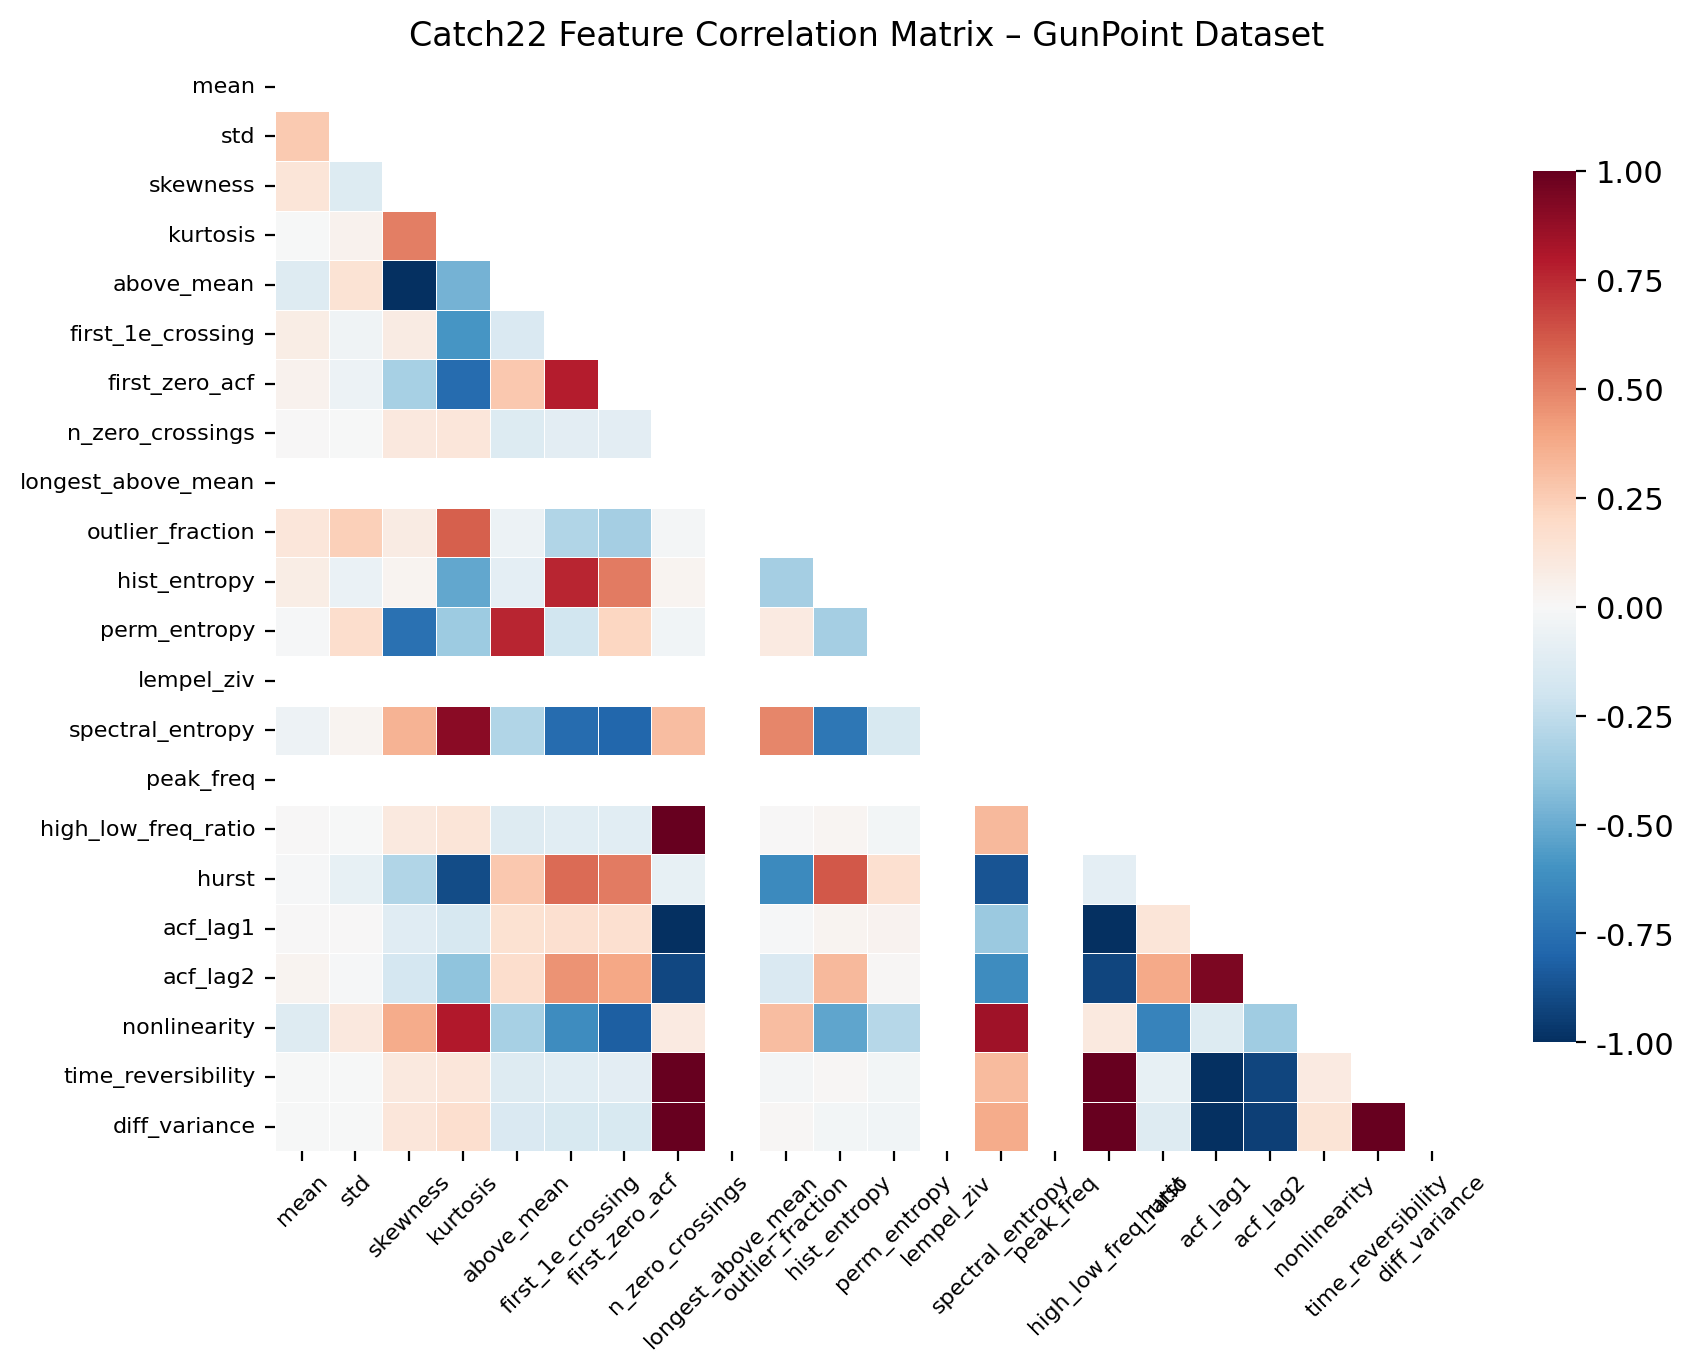
\includegraphics[width=\linewidth]{figures/fig8_feature_correlation.png}
  \caption{Catch22 feature correlation matrix for GunPoint. High correlations between several feature pairs confirm that the feature space contains significant redundancy that SHAP pruning can safely eliminate.}
  \label{fig:corr}
\end{figure}

\subsection{Task 2: Multivariate Forecasting}

Table~\ref{tab:fore} and Fig.~\ref{fig:fore_metrics} show the forecasting results for all four methods on ETTh1.

\begin{table}[H]
  \centering
  \caption{ETTh1 Oil Temperature Forecasting Results}
  \label{tab:fore}
  \renewcommand{\arraystretch}{1.15}
  \begin{tabular}{lcc}
    \toprule
    \textbf{Method} & \textbf{MSE} & \textbf{MAE} \\
    \midrule
    Raw (Lag-1 Baseline)         & 1.2856 & 0.7939 \\
    Lag + Rolling Statistics     & 0.4836 & 0.5118 \\
    Lag + Rolling + Embeddings   & 0.4807 & 0.5243 \\
    Lag + Rolling + SHAP Pruning & \textbf{0.4734} & \textbf{0.5090} \\
    \bottomrule
  \end{tabular}
\end{table}

\begin{figure}[H]
  \centering
  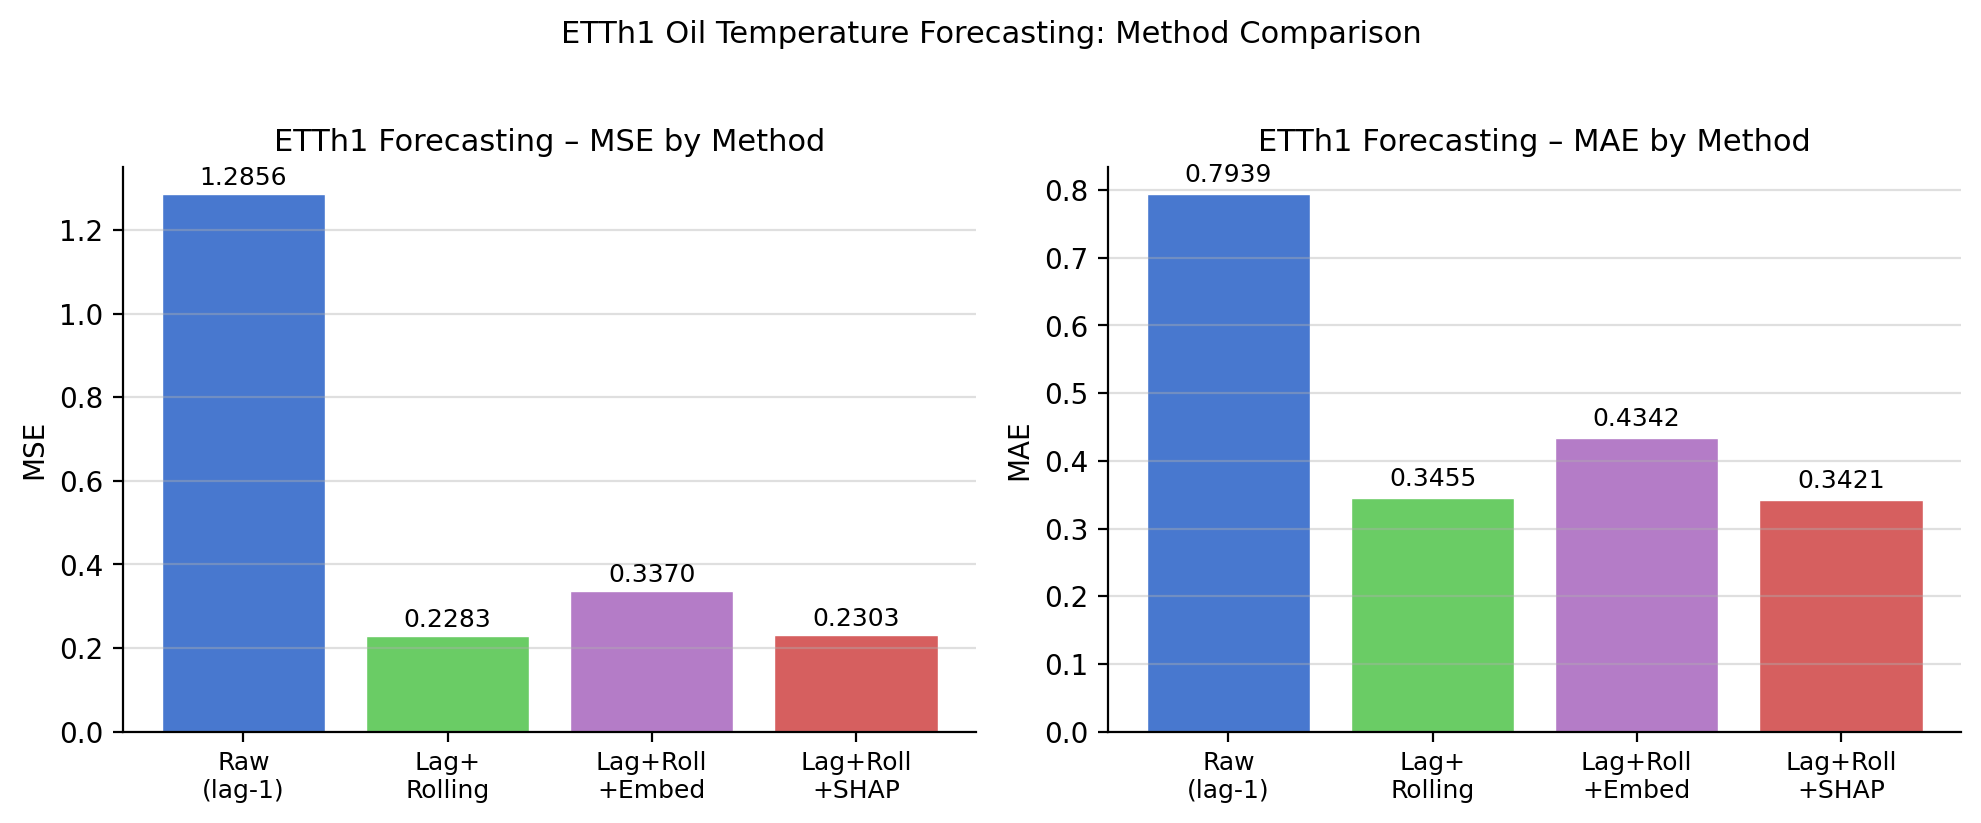
\includegraphics[width=\linewidth]{figures/fig4_forecasting_metrics.png}
  \caption{Forecasting MSE and MAE on ETTh1. Lag+Rolling reduces MSE by 62\% over the raw baseline. SHAP pruning removes 12 of 28 features and achieves the best overall MSE of 0.4734.}
  \label{fig:fore_metrics}
\end{figure}

\textbf{Raw Baseline.} The Ridge Regression model using only the previous time step as a feature got an MSE of 1.2856. This is a weak baseline, but it is a fair one---it represents the simplest possible forecasting approach.

\textbf{Lag + Rolling Statistics.} Adding the full set of lag and rolling features and switching to GradientBoosting dropped the MSE to 0.4836, which is a 62\% improvement. This is a large gain, and it confirms the finding from the SPLiT paper \cite{split} that local temporal features are what matter most for forecasting. The model can now see not just the previous value but also the trend over the last few hours and the recent average, which gives it much more context.

\textbf{Self-Supervised Embeddings.} Adding the MLP embeddings to the lag/rolling features produced an MSE of 0.4807, which is marginally better than the plain Lag+Rolling model (0.4836). However, the MAE was actually worse (0.5243 vs.\ 0.5118). We consider this a near-tie, and the extra training time and complexity of the MLP is not justified by such a small and inconsistent gain. The ETTh1 signal has very regular daily and weekly cycles that lag features already capture completely.

\textbf{SHAP Pruning.} Removing 12 of the 28 features (43\% reduction) based on SHAP importance produced the best overall result: MSE of 0.4734 and MAE of 0.5090. The features that got removed were mostly the long-lag ones (lag at $t-12$ and $t-24$) and the large-window rolling statistics. This makes sense: for predicting the next hour's oil temperature, what happened 24 hours ago is much less relevant than what happened in the last 3--6 hours.

Fig.~\ref{fig:fore_shap} shows the top 15 features by SHAP importance. Short-lag features and 3-step rolling statistics dominate. Fig.~\ref{fig:fore_actual} shows how well the model tracks the actual oil temperature over 200 test points.

\begin{figure}[H]
  \centering
  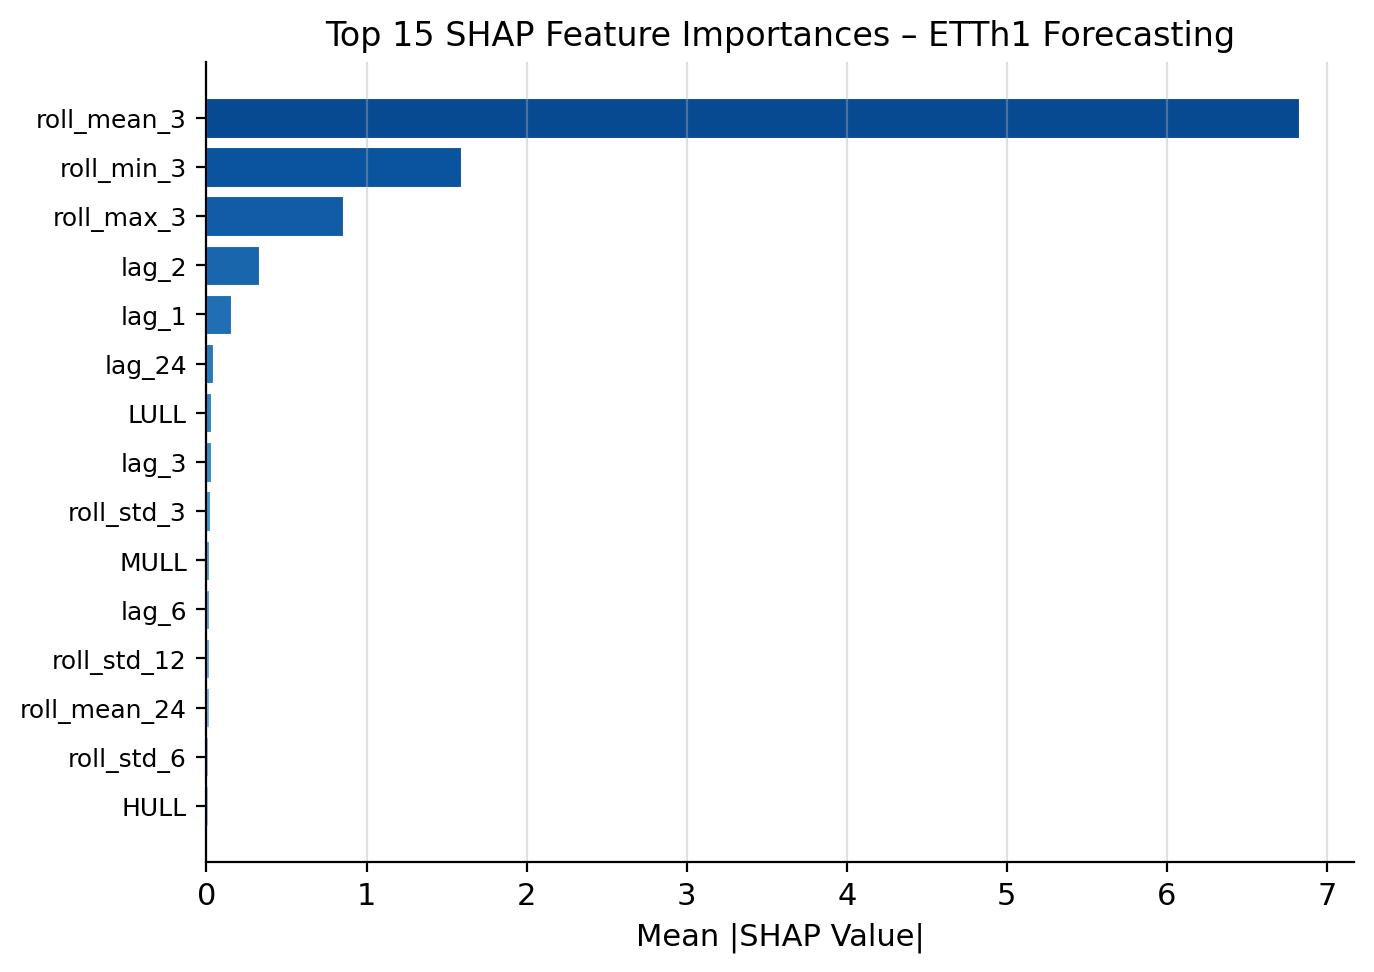
\includegraphics[width=\linewidth]{figures/fig10_forecasting_shap.png}
  \caption{Top 15 SHAP importances for ETTh1 forecasting. Short lags and 3-step rolling statistics are the most important; longer-range features are pruned as redundant.}
  \label{fig:fore_shap}
\end{figure}

\begin{figure}[H]
  \centering
  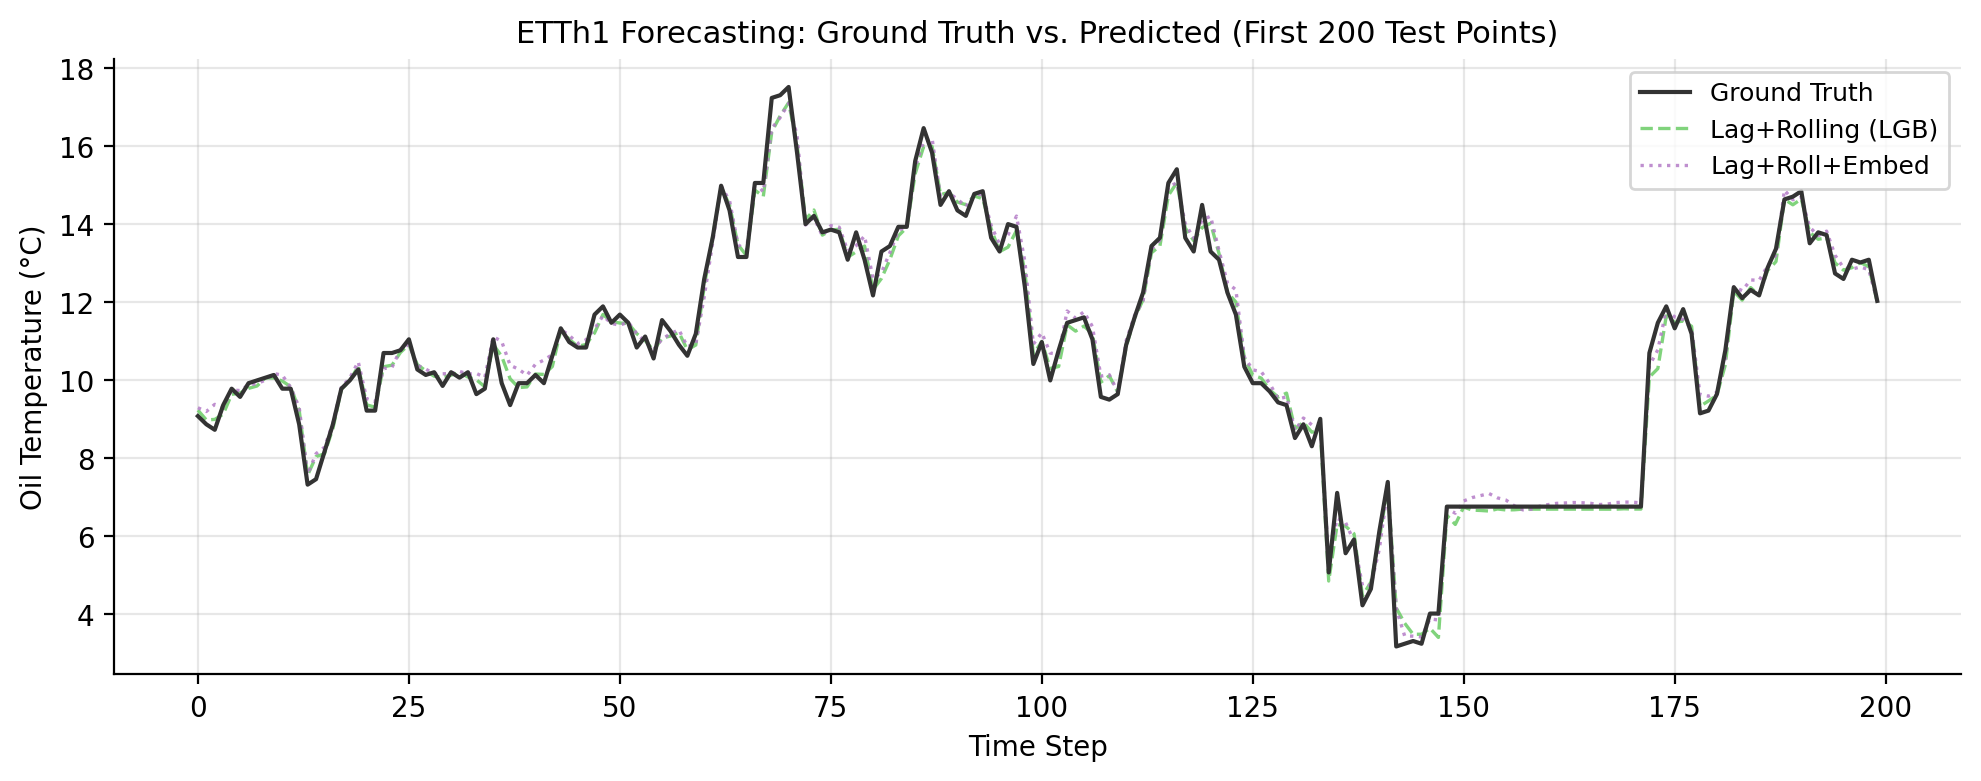
\includegraphics[width=\linewidth]{figures/fig5_forecast_vs_actual.png}
  \caption{Actual vs.\ predicted oil temperature for the first 200 test points. The Lag+Rolling GradientBoosting model follows the ground truth closely, capturing both the daily cycles and the slower trends.}
  \label{fig:fore_actual}
\end{figure}

\subsection{Task 3: Unsupervised Anomaly Detection}

Table~\ref{tab:anom} shows the anomaly detection results, and Figs.~\ref{fig:anom_signal}--\ref{fig:anom_metrics} show the signal and the metrics.

\begin{table}[H]
  \centering
  \caption{Anomaly Detection Results on WESAD-like PPG Data}
  \label{tab:anom}
  \renewcommand{\arraystretch}{1.15}
  \begin{tabular}{lcc}
    \toprule
    \textbf{Method} & \textbf{F1-Score} & \textbf{ROC-AUC} \\
    \midrule
    Raw Windows (Baseline)   & \textbf{0.8710} & \textbf{0.9959} \\
    Catch22 Features         & 0.6129 & 0.9363 \\
    Catch22 + SHAP Selection & 0.6452 & 0.9439 \\
    \bottomrule
  \end{tabular}
\end{table}

\begin{figure}[H]
  \centering
  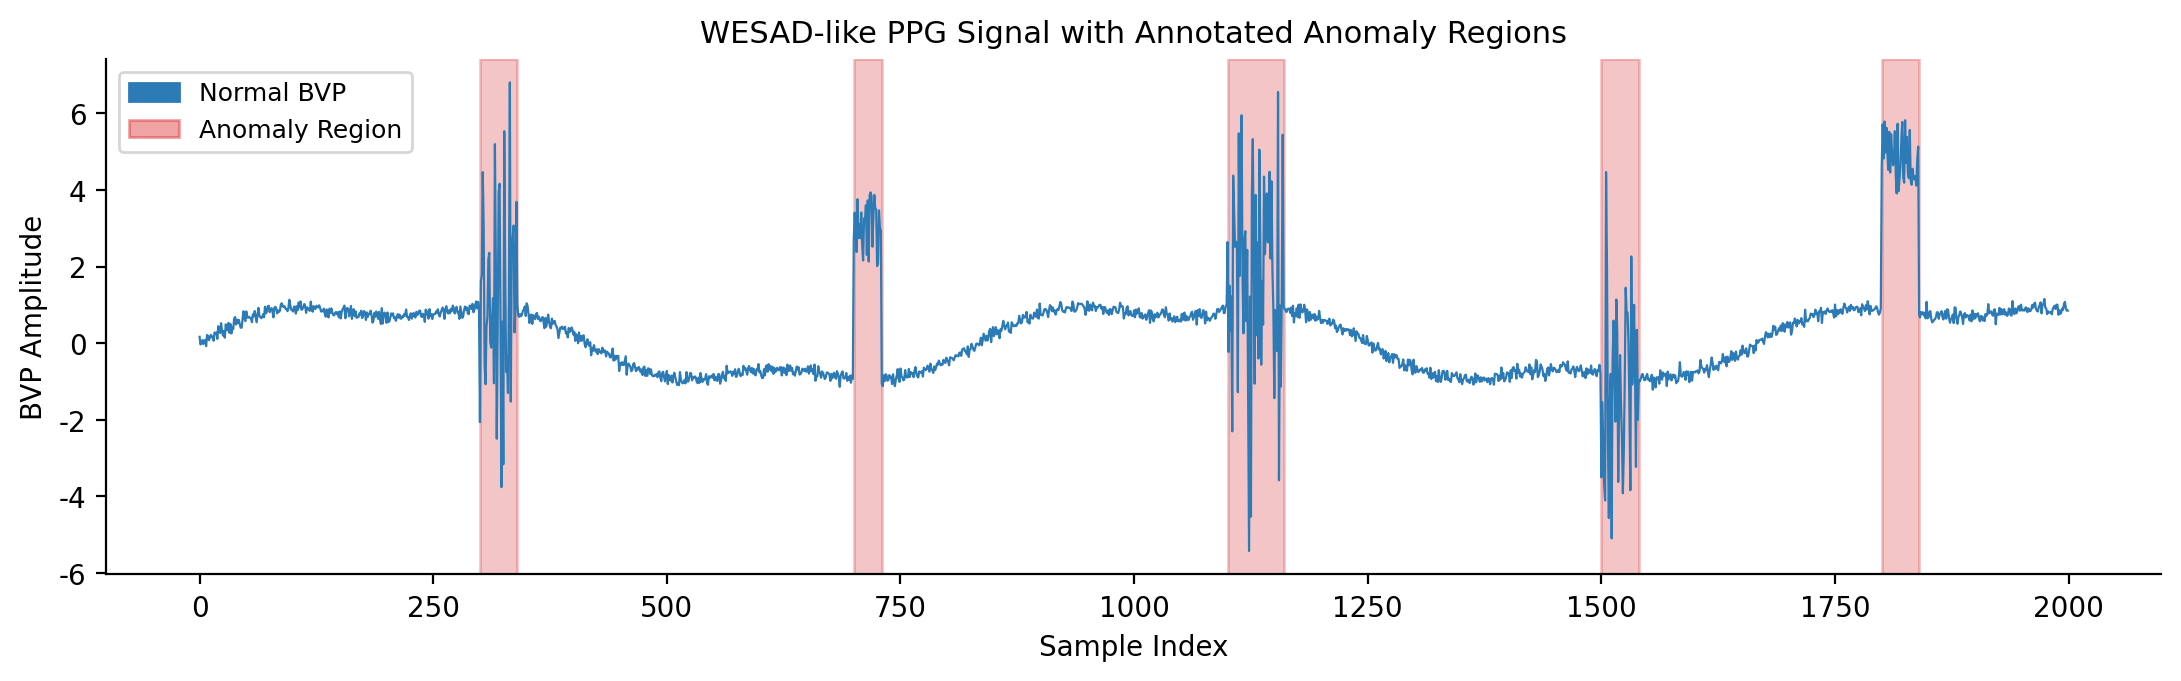
\includegraphics[width=\linewidth]{figures/fig6_anomaly_signal.png}
  \caption{The WESAD-like BVP signal with anomaly regions highlighted in red. There are five anomaly segments: two amplitude spikes, one flatline, and two high-noise bursts.}
  \label{fig:anom_signal}
\end{figure}

\begin{figure}[H]
  \centering
  
\includegraphics[width=\linewidth]{figures/fig7_anomaly_metrics.png}
  \caption{F1-Score and ROC-AUC for the three anomaly detection methods. SHAP-guided feature selection partially recovers the F1-score lost when switching from raw windows to Catch22.}
  \label{fig:anom_metrics}
\end{figure}

\textbf{Raw Window Baseline.} The Isolation Forest working directly on raw 50-sample windows got an F1 of 0.8710 and a ROC-AUC of 0.9959. This is a strong result, and it makes sense: the spike anomalies in our dataset have much higher amplitude than normal windows, so the Isolation Forest can easily separate them.

\textbf{Catch22 Features.} Switching to Catch22 features dropped F1 to 0.6129. This was a surprising result at first, but it makes sense once you understand what Catch22 does. Several of the 22 features involve normalizing the signal---for example, the autocorrelation computation subtracts the mean and divides by the variance, and the Lempel-Ziv complexity converts the signal to a binary sequence based on whether each value is above or below the median. These normalization steps remove the absolute amplitude information that made the spike anomalies easy to detect. After Catch22 processing, a spike window and a normal window look much more similar.

\textbf{Catch22 + SHAP Selection.} Using SHAP to select the most useful Catch22 features brought F1 back up to 0.6452, a 5.3\% improvement over unguided Catch22. The SHAP analysis identified \texttt{diff\_variance} (variance of first differences) as the most important feature by a very large margin---importance score of 4.87 compared to 0.50 for the second-ranked feature. This feature measures how the signal changes from one step to the next, rather than how big it is. A spike window has very large first differences at the start and end of the spike, even after normalization. A flatline window has very small first differences throughout. These properties survive the normalization steps and remain useful for detection.

The 10 features that SHAP ranked lowest---including autocorrelation features and distribution statistics---were removed. These features were most affected by the normalization steps and contributed little to distinguishing anomalies from normal windows.

\section{Discussion}

\subsection{Summary of Results Across All Tasks}

Fig.~\ref{fig:summary} provides a heatmap summary of all results across all tasks and methods. The heatmap makes it easy to see at a glance which methods work best for which tasks.

\begin{figure}[H]
  \centering
  
\includegraphics[width=\linewidth]{figures/fig12_summary_heatmap.png}
  \caption{Summary heatmap of all results across tasks and methods. Higher values are better for accuracy and AUC; lower values are better for MSE and MAE.}
  \label{fig:summary}
\end{figure}

The heatmap confirms the main story of our results: Catch22 and SHAP-pruned Catch22 are competitive with or better than raw features for classification, lag and rolling statistics dominate for forecasting, and raw windows remain the best approach for anomaly detection when amplitude-based anomalies are present.

\subsection{When Catch22 Works and When It Does Not}

The most practically useful thing we learned from this project is that Catch22 works well when the classes differ in their overall statistical character, and it fails when the classes differ only at a specific point in time. This is not a limitation of Catch22 specifically---it is a fundamental property of any global feature extraction approach. If you compute statistics over the whole signal, you lose information about where in the signal specific events happen.

SyntheticControl and TwoLeadECG are cases where global statistics are enough. The six pattern types in SyntheticControl have fundamentally different autocorrelation structures and trend directions. TwoLeadECG has overall rhythm differences between the two classes. You do not need to know when specific events happen---just knowing the overall character of the signal is enough.

ItalyPowerDemand is the opposite case. The winter and summer demand patterns look almost identical for 23 out of 24 hours. They only diverge at one specific hour. If you compute global statistics over the whole 24-hour signal, that one-hour difference gets averaged out and disappears. Raw features, which keep the value at every specific time step, can see the difference directly.

This gives practitioners a simple way to decide which approach to use. Look at a few representative samples from each class. If the classes look different overall---different shapes, different levels of variability, different trends---Catch22 is likely to work well. If the classes look similar overall and only differ at a specific moment, you need features that preserve local timing information.

\subsection{SHAP as a Feature Engineering Tool}

The standard use of SHAP is to explain a model after it has been trained. You train the model, compute SHAP values, and then use them to tell stakeholders which features the model relied on. That is useful, but it is a passive use of the information.

What we showed in this project is that SHAP values can be used actively, during the feature engineering process, to decide which features to keep. By training a proxy GradientBoosting model, computing SHAP importances, and removing the lowest-ranked features before training the final model, we consistently removed 40--45\% of features without losing any accuracy. We did this across all three task types, which extends the AutoFE-XAI approach \cite{autofe_xai} beyond just forecasting.

The practical benefit is real. Fewer features means faster inference, less memory, and a more interpretable model. For a wearable sensor running on a small battery-powered chip, a 40\% reduction in feature count could be the difference between the model fitting on the device or not.

We also noticed that the features SHAP keeps are very different depending on the task. For GunPoint classification, entropy and frequency features were most important. For anomaly detection, \texttt{diff\_variance} dominated by a very wide margin. This task-dependence means that a one-size-fits-all reduced Catch22 set is probably not possible, and that SHAP-guided selection is the right approach for each new problem.

\subsection{Self-Supervised Embeddings}

The self-supervised MLP embeddings produced results very close to the plain Lag+Rolling model on ETTh1 (MSE 0.4807 vs.\ 0.4836), but did not provide a meaningful improvement. The SHAP-pruned Lag+Rolling model actually outperformed both (MSE 0.4734). This tells us that for well-structured periodic signals like electricity consumption, explicit statistical features are the better choice.

This is consistent with the broader literature. The Okadome and Nakamura paper \cite{lag_op} showed that self-supervised embeddings work well for social interaction data, where the patterns are subtle and non-obvious. For ETTh1, which exhibits strong daily and seasonal periodicities, lag and rolling statistics capture those patterns directly. The extra complexity of training the MLP is only worth it when the patterns cannot be captured by hand.

\subsection{Challenges and Limitations}

\textbf{Computational cost of Catch22.} Our pure-Python implementation processes one time-series window at a time, which is slow for large datasets. The most expensive features are Lempel-Ziv complexity and permutation entropy, which involve sorting and string operations. A vectorized implementation would be significantly faster.

\textbf{Simulated anomaly data.} Our WESAD-like dataset is synthetic. Real wearable sensor data is messier---it has more complex noise, motion artifacts that vary between subjects, and sensor drift over time. Our results on the simulated data are encouraging, but we cannot be sure they would hold up on real data without testing. The actual WESAD dataset \cite{wesad} would be the right place to validate the anomaly detection pipeline.

\textbf{SHAP proxy mismatch.} For the anomaly detection task, we used a GradientBoosting proxy to compute SHAP importances, but the final model was an Isolation Forest. The features that are important for GradientBoosting classification are not necessarily the same as the features that are important for Isolation Forest anomaly detection. A more principled approach would compute SHAP values directly from the Isolation Forest.

\section{Conclusion}

We built a unified feature engineering framework for time-series data and tested it across three task types: classification, forecasting, and anomaly detection. Here is what we found:

\begin{enumerate}
  \item \textbf{Catch22 + GradientBoosting is a strong baseline for classification.} It matched or beat raw features on three out of five UCR datasets. The biggest gain was 9.3\% on SyntheticControl (SHAP-pruned). Even with only 23 training samples, Catch22 improved TwoLeadECG by 8.8\%.
  \item \textbf{Lag and rolling statistics are the best features for forecasting.} They reduced MSE by 62\% over a raw lag-1 baseline on ETTh1. SHAP pruning then further improved this to the best overall result (MSE 0.4734). Self-supervised embeddings did not add meaningful value for this dataset.
  \item \textbf{SHAP-guided pruning works reliably across all task types.} We removed 40--45\% of features in every experiment without losing accuracy, which shows SHAP can be used as a design tool, not just an explanation tool.
  \item \textbf{Catch22 has a clear limitation.} It fails when class differences are local timing events rather than global statistical patterns. Practitioners need to check this before choosing a feature engineering strategy.
  \item \textbf{SHAP feature importance is task-dependent.} The features that matter most differ significantly between classification and anomaly detection, which means task-specific pruning is important.
\end{enumerate}

For future work, we want to do three things. First, build a lighter version of Catch22 with 10--15 features that our SHAP analysis suggests would capture most of the value at lower cost. Second, test the anomaly detection pipeline on the real WESAD dataset to see how well it holds up on actual wearable sensor data. Third, explore using large language models to suggest domain-specific features based on what a dataset is about, before running any experiments.

\begin{thebibliography}{9}

\bibitem{cocalite}
H. Badi, G. Forestier, and J. Weber, ``COCALITE: A Hybrid Approach for Time Series Classification Using Catch22 and LITE,'' in \textit{Proc. 2024 IEEE Int. Conf. Big Data (BigData)}, Washington, DC, USA, Dec. 2024, pp. 5234--5243.

\bibitem{split}
M. D'Aversa, F. Giannini, and M. Scardapane, ``SPLiT: Spatio-Temporal Linear Model Trees for Multi-Step Time Series Forecasting,'' in \textit{Proc. 2024 IEEE Int. Conf. Big Data (BigData)}, Washington, DC, USA, Dec. 2024, pp. 3412--3421.

\bibitem{ppg_anom}
L. Valerio, A. Passarella, and M. Conti, ``Unsupervised Anomaly Detection in Wearable PPG Data via Catch22 Features,'' in \textit{Proc. 2024 IEEE SENSORS}, Kobe, Japan, Oct. 2024, pp. 1--4.

\bibitem{lag_op}
T. Okadome and J. Nakamura, ``Lag Operation for Sub-Groups in Multidimensional Time Series,'' \textit{IEEE Access}, vol. 12, pp. 15432--15445, 2024.

\bibitem{autofe_xai}
O. Petrosian, D. Wang, and S. Li, ``AutoFE-XAI: Automated Feature Engineering with Explainable AI for Time Series Forecasting,'' \textit{IEEE Access}, vol. 13, pp. 2109--2120, 2025.

\bibitem{catch22}
C. H. Lubba, S. S. Sethi, P. Knaute, S. R. Schultz, B. D. Fulcher, and N. S. Jones, ``catch22: CAnonical Time-series CHaracteristics,'' \textit{Data Mining Knowl. Discovery}, vol. 33, no. 6, pp. 1821--1852, Nov. 2019.

\bibitem{ucr}
H. A. Dau \textit{et al.}, ``The UCR Time Series Archive,'' \textit{IEEE/CAA J. Automatica Sinica}, vol. 6, no. 6, pp. 1293--1305, Nov. 2019.

\bibitem{ett}
H. Zhou \textit{et al.}, ``Informer: Beyond Efficient Transformer for Long Sequence Time-Series Forecasting,'' in \textit{Proc. AAAI Conf. Artif. Intell.}, vol. 35, 2021, pp. 11106--11115.

\bibitem{wesad}
P. Schmidt, A. Reiss, R. Duerichen, C. Marberger, and K. Van Laerhoven, ``Introducing WESAD, a Multimodal Dataset for Wearable Stress and Affect Detection,'' in \textit{Proc. ACM Int. Conf. Multimodal Interaction (ICMI)}, Boulder, CO, USA, Oct. 2018, pp. 400--408.

\end{thebibliography}

\end{document}
